\section{Cours 6}\label{cours-6}

\subsection{Course à la performance}\label{course-uxe0-la-performance}

Selon la loi empirique de Moore, tous les 18 mois, la quantité de
transistor sur \(1\) \(cm^2\) double.

\subsubsection{Horloge}\label{horloge}

On sait que les processeurs fonctionnent sur des cycles régulés par
l'horloge. On voit apparaître un plateau vers 2001 pour les fréquences
d'horloge.

\paragraph{Raison}\label{raison}

\begin{itemize}
\tightlist
\item
  \emph{Memory Wall}: la différence entre fréquence CPU et RAM est trop
  importante. Demande plus de cache mais c'est cher
\item
  \emph{Instruction-Level Parallelism}: Même si possible de paralléliser
  les processus, on reste limité par les instructions bas niveaux.
\item
  \emph{Power Wall}: + de fréquence = + de consommation d'énergie = + de
  dissipation thermique. Cela devient compliqué à refroidir.
\end{itemize}

\subsubsection{Augmentation des
performances}\label{augmentation-des-performances}

\begin{figure}
\centering
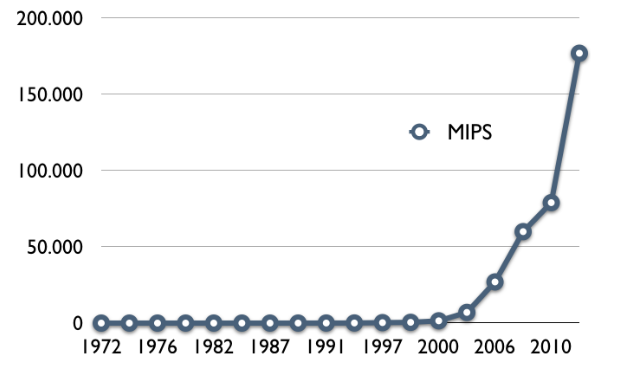
\includegraphics{image-22.png}
\caption{Alt text}
\end{figure}

On voit bien que le \emph{Millions d'Instructions par Seconde} augmente
tout de même.

Ces résultats sont démontrés via des \textbf{benchmarks standardisés}.
(SPEC = organisation de standardisation de benchmarks)

\paragraph{Multi-coeurs}\label{multi-coeurs}

C'est grâce au multi-coeurs ! Le nombre de transistor augmente mais la
fréquence est stable donc le nombre d'instructions par seconde augmente.

On peut ainsi avoir plusieurs \textbf{threads} qui s'exécutent en
simultanée.

\begin{figure}
\centering
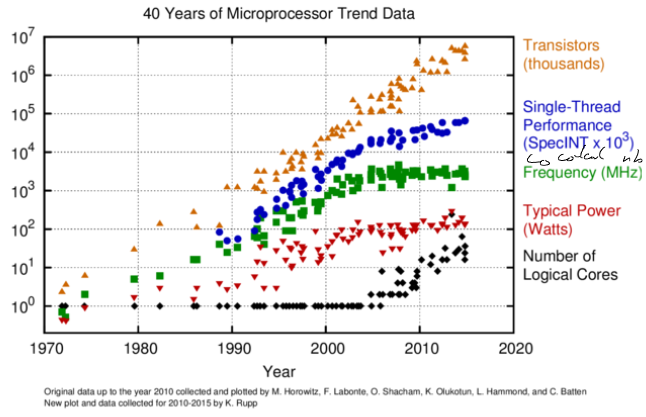
\includegraphics{image-23.png}
\caption{Alt text}
\end{figure}

On ne remplit pas totalement tous les coeurs via un seul programme car
il manque de parallélisme d'instruction (ILP).

Les ressources du coeur sont partagées entre 2 fils d'instructions
distincts: - \textbf{SMT}: \emph{Simultaneous Multi-Threading} - 32 fils
par coeur sur certains CPU - 2 fils par coeur souvent
(\emph{Hyperthreading})

Un peu inférieur: 16 threads \textless{} 16 coeurs

\subsection{Threads}\label{threads}

\subsubsection{Qu'est-ce qu'un thread ?}\label{quest-ce-quun-thread}

Un threads est donc: 1. Instructions à exécuter (text) 2. Mémoires
contenant les données manipulées (\emph{data, heap, stack}) 3. Registres
du CPU (son état actuel)

\subsubsection{Mise en oeuvre (POSIX)}\label{mise-en-oeuvre-posix}

Avec les threads POSIX: \emph{threads du programme utilisateur = threads
ordonnancé sur les coeurs par le noyau}. En gros le gain des threads
POSIX se fait sentir jusqu'à ce que le nombre de threads du programme
atteignent ceux du CPU (cfr: Projet 3).

\paragraph{Utilisation}\label{utilisation}

On utilise la libraire \texttt{pthreads(7)} et à la compilation on doit
passer le flag \texttt{-lpthread} à gcc.

\begin{Shaded}
\begin{Highlighting}[]
\PreprocessorTok{\#include }\ImportTok{\textless{}pthread.h\textgreater{}}

\DataTypeTok{int}\NormalTok{ pthread\_create}\OperatorTok{(}\NormalTok{pthread\_t }\OperatorTok{*}\DataTypeTok{restrict}\NormalTok{ thread}\OperatorTok{,}
                   \DataTypeTok{const}\NormalTok{ pthread\_attr\_t }\OperatorTok{*}\DataTypeTok{restrict}\NormalTok{ attr}\OperatorTok{,}
                   \DataTypeTok{void} \OperatorTok{*(*}\NormalTok{start\_routine}\OperatorTok{)(}\DataTypeTok{void} \OperatorTok{*),}
                   \DataTypeTok{void} \OperatorTok{*}\DataTypeTok{restrict}\NormalTok{ arg}\OperatorTok{);}
\end{Highlighting}
\end{Shaded}

\begin{itemize}
\tightlist
\item
  \texttt{thread}: structure de donnée provenant de \texttt{pthread.h}
\item
  attributs: \texttt{NULL} par défaut
\item
  \texttt{start\_routine}: pointeur sur la fonction, point de départ du
  thread
\item
  \texttt{arg}: arguments à passer à notre fonction de
  \texttt{start\_routine}
\end{itemize}

Retourne \(0\) si aucune erreur.

\paragraph{Récupérer la valeur de
retour}\label{ruxe9cupuxe9rer-la-valeur-de-retour}

\begin{Shaded}
\begin{Highlighting}[]
\PreprocessorTok{\#include }\ImportTok{\textless{}pthread.h\textgreater{}}

\DataTypeTok{int}\NormalTok{ pthread\_join}\OperatorTok{(}\NormalTok{pthread\_t thread}\OperatorTok{,} \DataTypeTok{void} \OperatorTok{**}\NormalTok{value\_ptr}\OperatorTok{);}
\end{Highlighting}
\end{Shaded}

\begin{itemize}
\tightlist
\item
  \texttt{thread}: thread concerné.
\item
  \texttt{value\_ptr}: pointeur où on va récupérer la valeur.
\end{itemize}

\texttt{pthread\_join} ne retourne qu'à la terminaison du thread. Donc
on attend jusqu'à la fin de son exécution.

\paragraph{Fonctionnement}\label{fonctionnement}

Au moment d'exécuter \texttt{pthread\_create} la pile du thread est
créée et la valeur de l'argument y est copié. Donc on doit s'assurer que
le pointeur passé soit toujours valide à n'importe quel moment. Moment
de l'exécution du thread inconnu.

Dans un thread, il a un nouveau stack et contexte (\%esp, \%eip,
registres). Cependant il utilise le heap, les données statiques et le
text du processus principal.

\subsubsection{Communication entre
thread}\label{communication-entre-thread}

On va utiliser des locks pour pouvoir accéder à des variables globales
sans se marcher dessus.

On doit d'abord s'assurer de gérer les interruptions pour les
\textbf{changements de contexte}. On fait cela via: - Appel système
bloquant - Réception d'une interruption: - Signal électronique reçu par
le processeur pour signaler la disponibilité d'une E/S - Ou via un timer
régulier.

Appel bloquant comme \texttt{getchar} qui attend une entrée utilisateur.

\subsubsection{États}\label{uxe9tats}

\begin{figure}
\centering
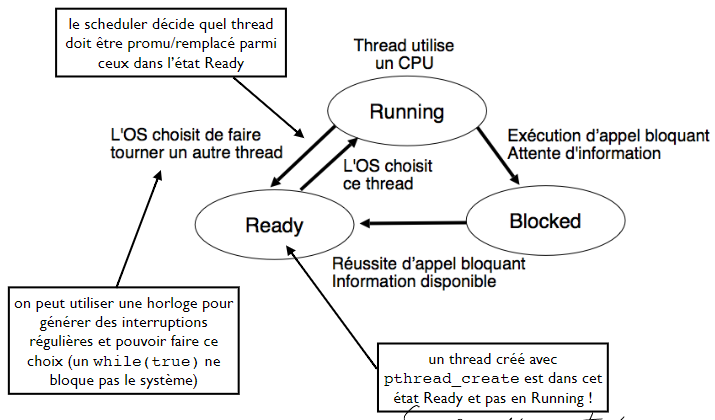
\includegraphics{image-24.png}
\caption{Alt text}
\end{figure}

\paragraph{Laisser la main}\label{laisser-la-main}

Un thread peut libérer le processeur via \texttt{pthread\_yield} pour ne
pas bloquer (appel sys bloquant \texttt{sleep}/\texttt{usleep}).

Il faut faire attention au blocage de la machine suite à l'arrêt des
entrées/sorties.

\subsubsection{MUTEX}\label{mutex}

C'est un objet qui va être \textbf{unlocked} si on peut y accéder et
\textbf{locked} si on ne peut pas. On utilise les fonctions
\texttt{lock()} et \texttt{unlock()}.

Si un thread appelle \texttt{lock()} et que le mutex est déjà bloqué,
alors le thread sera interrompu et placé en mode \textbf{Blocked}
jusqu'à ce que le mutex soit libéré. \texttt{lock()} peut créer un appel
sys bloquant.

\paragraph{Deadlock}\label{deadlock}

cela se passe quand tout se bloque à cause de mutex (cfr: 3 philosophes
3 baguettes). On peut forcer que les appels bloquants se fassent par
ordre croissant d'adresse pour éviter ce problème.
